\chapter{\IfLanguageName{dutch}{Stand van zaken}{State of the art}}%
\label{ch:stand-van-zaken}

% Tip: Begin elk hoofdstuk met een paragraaf inleiding die beschrijft hoe
% dit hoofdstuk past binnen het geheel van de bachelorproef. Geef in het
% bijzonder aan wat de link is met het vorige en volgende hoofdstuk.

% Pas na deze inleidende paragraaf komt de eerste sectiehoofding.

\section{Inleiding tot aanbevelingssystemen}
Aanbevelingssystemen zijn algoritmes en software tools met als doel om gepersonaliseerde aanbevelingen op basis van gelijkenis van items, gebruikersprofiel of andere kenmerken, te geven aan gebruikers \autocite{Patel2020, Patel2023}. De aanbevelingen worden gemaakt aan de hand van verschillende besluitvormingsprocessen, zoals welk nieuws hij leest, naar welke film hij kijkt of naar welke muziek hij luistert \autocite{Patel2017}. De kernfunctie van een aanbevelingssysteem is het voorspellen van de relevantie of voorkeur die een gebruiker aan een item zou toekennen, waarbij de enorme hoveelheid informatie gefilterd wordt en gebruikers enkel keuzes krijgen voorgeschoteld die op hun interesses zijn afgestemd \autocite{Fkih2022}. Anders gezegd kunnen aanbevelingssystemen gezien worden als functies die informatie over de voorkeuren van een gebruiker (bijv. over films) als invoer nemen en een voorspelling doen over de beoordeling die een gebruiker zou geven aan andere gewenste items (bijv. nieuwe beschikbare films) en het uitvoer zijn aanbevelingen van deze items \autocite{Milano2020}. Aanbevelingen kunnen gaan over een breed scala aan items, waaronder producten in e-commerce, films, muziek, nieuwsartikelen en contacten op sociale media.
\subsection{Toepassingen van aanbevelingssystemen}
De toepassingen van aanbevelingssystemen zijn uitgebreid en doordringen talloze domeinen. Een van de meeste bekende toepassing is in e-commerce, waar producten aanbevelen aan klanten op basis van hun aankoopgeschiedenis en surfgedrag, zoals de Amazon \"item-to-item \ac{cf}\" algoritme \autocite{Patel2023, Patel2020}.

In de entertaintment industrie bij het aanbevelen van films op Netflix, IMDB of MovieLens en muziek \autocite{Patel2020, Roy2022}. Op sociale media platformen zoals Facebook en Twitter worden aanbevelingen gedaan voor nieuwe personen en pagina's te ontdekken \autocite{Patel2023}. Zelfs de advertenties op deze platformen zijn vaak afgestemd op de intresses van de gebruiker \autocite{Patel2020}.

In het onderzoek \textcite{Agapito2016} wordt DIETOS (DIET Organizer System) geïntroduceerd, een webgebaseerd aanbevelingssysteem dat gepersonaliseerd voedingsadvies biedt op basis van een gezondheidsprofiel van de gebruiker. Dit profiel wordt opgebouwd via dynamische vragenlijsten die zijn ontwikkeld en gevalideerd door medische professionals. Het systeem richt zich specifiek op het aanbevelen van geschikte voedingsmiddelen voor personen met chronische aandoeningen zoals diabetes, hypertensie en chronische nierziekten. Toeristen kunnen ook geholpen worden bij het plannen van hun reis door aanbevelingen te geven over bezienswaardigheden, restaurants en hotels \autocite{Roy2022, Patel2023}.
\subsection{Wat maakt ze nuttig?}
Tegenwoordig wordt overweldigende data geproduceerd waardoor gebruikers makkelijk overbeslast kunnen worden met informatie en keuzes. Een gebruiker zou zelf door de data moeten filteren om het gewenst item te vinden. Aanbevelingssystemen bieden een oplossing voor dit probleem door data te analyseren en te filteren om nuttige informatie te extraheren \autocite{Fkih2022}. Ze zijn in staat om gebruikersvoorkeuren en gedrag te voorspellen waardoor ze kunnen inspelen op de behoeften van de gebruiker \autocite{Mazeh2020}. Ze verbeteren de besluitvorming van gebruikers door relevante opties voor te stellen, zoals wat te kopen, te lezen of te bekijken, en moedigen hen aan om actie te ondernemen \autocite{Mazeh2020}. Daarnaast spelen aanbevelingssystemen een belangrijke rol in het creëren van bedrijfswaarde, doordat ze bijdragen aan verkoop en omzet door producten aan te bevelen die klanten waarschijnlijk zullen kopen \autocite{Wang2018, Patel2023}. \autocite{MacKenzie2013} toont aan dat 35\% van de aankopen op Amazon en 75\% van wat gebruikers op Netflix bekijken, te danken is aan gepersonaliseerde aanbevelingen. Huidige cijfers zijn waarschijnlijk nog hoger.
\subsection{Soorten aanbevelingssystemen}
Er bestaan verschillende typen aanbevelingssystemen waarvan de meest voorkomende zijn:
\begin{itemize}
  \item \textbf{Content-based Filtering (CBF)}: Deze methode beveelt items aan die vergelijkbaar zijn met items die een gebruiker in het verleden heeft gewaardeerd of waarmee hij/zij heeft geïnterpreteerd. Het systeem analyseert de eigenschappen of beschrijvingen van items (bijv. genre, trefwoorden of metadata) en matcht deze met het interesseprofiel van de gebruiker \autocite{Patel2023}.
  \begin{figure}
    \centering
    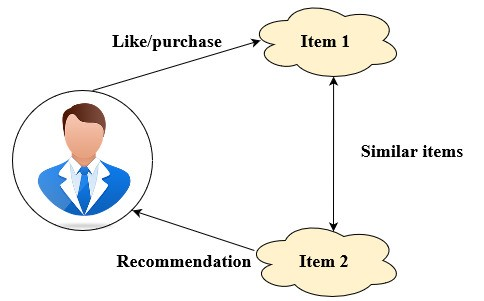
\includegraphics[width=0.4\textwidth]{cb-rs-patel2023.jpg}
    \caption[Content-based Filtering aanbevelingssysteem]{\label{fig:CBFRS} Visualitie hoe een aanbevelingssysteem met de CBF benadering aanbevelingen doet \autocite{Patel2023}}
  \end{figure}
  \item \textbf{Collaborative Filtering (CF)}: Dit type maakt aanbevelingen op basis van de voorkeuren en het gedrag van andere gebruikers met vergelijkbare smaken. Het identificeert gebruikers met vergelijkbare eerdere interacties (gebruikersgebaseerd) of items die vaak samen worden gewaardeerd (itemsgebaseerd) en beveelt items aan die deze gebruikers leuk vonden \autocite{Patel2023}. Dit kan verder worden onderverdeeld in twee categorieën, gebaseerd op geheugen (memory-based) en model (model-based).
  \begin{figure}
    \centering
    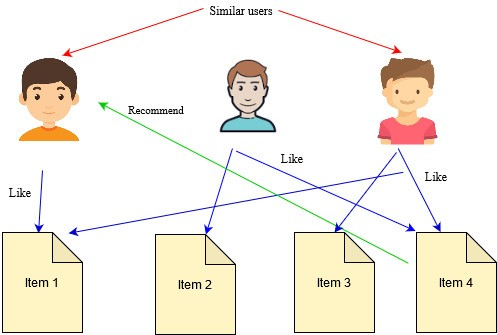
\includegraphics[width=0.4\textwidth]{cf-rs-patel2023.jpg}
    \caption[Collaborative Filtering aanbevelingssysteem]{\label{fig:CFRS} Visualitie hoe een aanbevelingssysteem met de CF benadering aanbevelingen doet \autocite{Patel2023}}
  \end{figure}
  \item \textbf{Hybride Filtering (HF)}: Hybride systemen combineren de sterke punten van content-based en collaborative filtering om de beperkingen van beide methoden te overwinnen. Door beide benaderingen te integreren, kunnen ze robuustere, nauwkeurigere en diversere aanbevelingen bieden \autocite{Patel2023}.
\end{itemize}
Naast deze hoofdcategorieën bestaan er ook andere soorten aanbevelingssystemen, waaronder:
\begin{itemize}
  \item \textbf{Knowledge gebaseerde systemen}: Deze systemen gebruiken expliciete kennis over gebruikers en items om te bepalen welke items aan de behoeften van een gebruiker voldoen \autocite{Patel2023}.
  \item \textbf{Demographic gebaseerde systemen}: Ze geven aanbevelingen op basis van de demografische profielen van gebruikers \autocite{Patel2023}.
  \item \textbf{Sequential aanbevelingssystemen}: Deze houden rekening met de volgorde van eerdere interacties van een gebruiker om te voorspellen waar hij/zij mogelijk in geïnteresseerd is \autocite{Patel2023, Zangerle2022}.
  \item \textbf{Session gebaseerde systemen}: Deze aanbevelingssystemen gebruiken algoritmen om gebruikers aanbevelingen te geven op basis van hun meest recente interacties tijdens de huidige sessie. Deze interacties kunnen verschillende vormen aannemen, zoals de browsegeschiedenis, klikgedrag, toegangstijd en andere acties die de gebruiker tijdens de sessie uitvoert. Een belangrijke verschil met traditionele aanbevelingssystemen is dat ze doorgaans geen rekening met de voorkeuren of gedragingen van gebruikers buiten de huidige sessie \autocite{Patel2023}. 
  \item \textbf{Context gebaseerde systemen}: Deze houden rekening met verschillende contextuele factoren, zoals tijd, locatie of de huidige situatie van de gebruiker, om relevantere aanbevelingen te bieden \autocite{Patel2023}.
  \item \textbf{Trustworthy Recommender Systems (TRSs)}: Een recente ontwikkeling die zich richt op aspecten zoals eerlijkheid, verklaarbaarheid, privacy en robuustheid bij het genereren van aanbevelingen \autocite{Wang2024}.
\end{itemize}
\begin{figure}
  \centering
  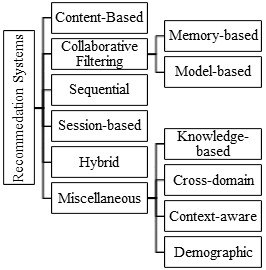
\includegraphics[width=0.4\textwidth]{taxonomie-rs-patel2023.jpg}
  \caption[Taxonomie van aanbevelingssystemen]{\label{fig:TaxonomieRS} Taxonomie van aanbevelingssystemen \autocite{Patel2023}}
\end{figure}
\subsection{Uitdagingen en ethische overwegingen van aanbevelingssystemen}
Aanbevelingssystemen bieden veel voordelen maar brengen ook enkele uitdagingen en ethische dilemma's met zich mee. Een van de meest urgente zorgen is privacy \autocite{Lex2023, Friedman2015, Li2017}. Het verzamelen en verwerken van gebruikersgegevens, die cruciaal zijn voor het genereren van effectieve aanbevelingen, kan resulteren in privacyschendingen en het onbedoeld blootleggen van gevoelige persoonlijke gegevens \autocite{Wang2018, Li2017}.

Een ander probleem is de zogenaamde filterbubbel, waarbij gebruikers alleen worden blootgesteld aan informatie die hun bestaande overtuigingen en vooroordelen bevestigt. Hierdoor komen ze in een echo-kamer terecht, waar ze geen toegang hebben tot diverse perspectieven en meningen. ndere ethische uitdagingen zijn onder meer het aanbevelen van ongepaste of twijfelachtige content, oneerlijkheid in aanbevelingen, en een gebrek aan transparantie over hoe aanbevelingen tot stand komen (ook wel "opaciteit" genoemd) \autocite{Milano2020}. Deze problemen kunnen de autonomie en identiteit van gebruikers ondermijnen en bestaande vooroordelen verder versterken.

Het cold-start probleem is een ander veelvoorkomend probleem bij aanbevelingssystemen, waarbij het systeem moeite heeft om aanbevelingen te doen voor nieuwe gebruikers of items die weinig interacties hebben gehad \autocite{Roy2022, Patel2023}. Datasparsheid komt daar in ook bij kijken doordat gebruikers-item interacties vaak beperkt zijn wordt het systeem opbouwen of trainen moeilijker \autocite{Roy2022, Patel2023}.

Gerelateerd aan trainen is het probleem van bias in de trainingsdata. Dit leidt tot ongelijke behandeling van gebruikers en items, wat kan resulteren in discriminerende aanbevelingen en het kan vooroordelen versterken. Eerlijkheid is een ander belangrijk aandachtspunt, zowel voor gebruikers (bijvoorbeeld door discriminatie te voorkomen) als voor items bijvoorbeeld door gelijke zichtbaarheid te bieden aan zowel populaire als minder populaire items \autocite{Wang2024}.

Een van de grootste technische uitdagingen is ervoor zorgen dat het systeem efficiënt en schaalbaar blijft. Naarmate het aantal gebruikers en producten toeneemt, moet het systeem snel en nauwkeurig blijven werken, wat veel rekenkracht vraagt \autocite{Roy2022, Patel2017}.

Daarom is voortdurend onderzoek en innovatie nodig om aanbevelingssystemen niet alleen effectief te houden, maar ook eerlijk, betrouwbaar en gebruiksvriendelijk te maken. 
\section{\ac{cf} gebaseerde aanbevelingssystemen}
\section{Toepassing \ac{fl} techniek}
\section{\ac{dp} framework}
\section{Evalueren van aanbevelingssystemen}

% \begin{figure}
%   \centering
%   \includegraphics[width=0.8\textwidth]{grail.jpg}
%   \caption[Voorbeeld figuur.]{\label{fig:grail}Voorbeeld van invoegen van een figuur. Zorg altijd voor een uitgebreid bijschrift dat de figuur volledig beschrijft zonder in de tekst te moeten gaan zoeken. Vergeet ook je bronvermelding niet!}
% \end{figure}

% \begin{listing}
%   \begin{minted}{python}
%     import pandas as pd
%     import seaborn as sns

%     penguins = sns.load_dataset('penguins')
%     sns.relplot(data=penguins, x="flipper_length_mm", y="bill_length_mm", hue="species")
%   \end{minted}
%   \caption[Voorbeeld codefragment]{Voorbeeld van het invoegen van een codefragment.}
% \end{listing}

\lipsum[7-20]

% \begin{table}
%   \centering
%   \begin{tabular}{lcr}
%     \toprule
%     \textbf{Kolom 1} & \textbf{Kolom 2} & \textbf{Kolom 3} \\
%     $\alpha$         & $\beta$          & $\gamma$         \\
%     \midrule
%     A                & 10.230           & a                \\
%     B                & 45.678           & b                \\
%     C                & 99.987           & c                \\
%     \bottomrule
%   \end{tabular}
%   \caption[Voorbeeld tabel]{\label{tab:example}Voorbeeld van een tabel.}
% \end{table}

